\begin{example}
    \begin{figure}
        \centering
        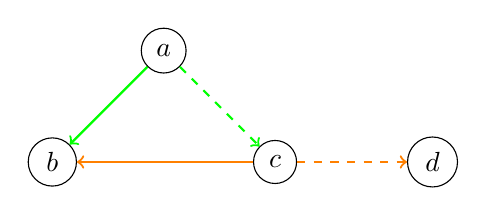
\begin{tikzpicture}[
                node distance={20mm},
                main/.style = {draw, circle},
                s/.style = {->,thick},
                d/.style = {->,thick,dashed} ]
            \node[main] (b) {$b$};
            \node[main] (a) [above right of=b] {$a$};
            \node[main] (c) [below right of=a] {$c$};
            \node[main] (d) [right of=c] {$d$};
            \draw[thick,green,->] (a) -- (b);
            \draw[thick,green,->,dashed] (a) -- (c);
            \draw[thick,orange,->] (c) -- (b);
            \draw[thick,orange,->,dashed] (c) -- (d);
        \end{tikzpicture}
        \caption{}
        \label{fig:blacklist}
    \end{figure}
    We define the following programs:
    \begin{align*}
        N & = p_i q_i f_{ad} + q_i p_i f_{ad} \\
        C & = p_o \times q_o \\
        SDN & = (N \times C)\lceil \Lambda \\
        \Lambda & = \s{(p_i,p_o),(q_i,q_o),(f_{ad},*)}
    \end{align*}
    This program captures the update behavior of the network 
    figure \ref{fig:blacklist}.
    Assume that two updates, $p$ and $q$ happening in the network.
    $p$ replaces the path $ab$ with $ac$ and $q$ replaces
    the path $cb$ with $cd$.
    Let $C$ be the controller that concurrently sends commands for these
    updates, $p_o,q_o$.
    We use $p_i$ and $q_i$ for actions of receiving these commands and
    $f_{ad}$ for the action of forwarding a packet from $a$ to $d$.
    For simplicity, we do not consider any forwarding in the network 
    other than $f_{ad}$.
    Event structure of the $SDN$ has the configurations as depicted 
    in figure \ref{fig:blacklist:es}.
    Blacklisted nodes are nodes in the network that must not
    be reachable \cite{network-abstractions}.
    Let's assume the network in figure \ref{fig:blacklist} as
    an example where the node $d$ is blacklisted.
    For simplicity we assume that we require
    $d$ not reachable only from $a$.
    Thus, we consider the existence of configurations
    $\s{p_1,q_1,ad_1}$ and $\s{p_2,q_2,ad_2}$ in an event structure
    as a property violation.
    In this example we can prove that $C_{p_1,q_1} = \F$ is an 
    actual cause of the property violation.
    \begin{figure}
        \centering
        \begin{tikzpicture}
            \crd{0}{0}{$\emptyset$}
            \crd[left]{-2}{1}{$\s{p_1}$}
            \crd[left]{-2}{2}{$\s{p_1,q_1}$}
            \crd[left]{-2}{3}{$\s{p_1,q_1,ad_1}$}
            \crd[right]{2}{1}{$\s{q_2}$}
            \crd[right]{2}{2}{$\s{p_2,q_2}$}
            \crd[right]{2}{3}{$\s{p_2,q_2,ad_2}$}
            \draw [ultra thick] (-2,1) -- (-2,2);
            \draw [ultra thick] (-2,2) -- (-2,3);
            \draw [ultra thick] (0,0) -- (2,1);
            \draw [ultra thick] (0,0) -- (-2,1);
            \draw [ultra thick] (2,1) -- (2,2);
            \draw [ultra thick] (2,1) -- (2,3);
        \end{tikzpicture}
        \caption{}
        \label{fig:blacklist:es}
    \end{figure}

\end{example}